\chapter{Study I: Comorbidity Clustering in Ischemic Heart Disease}
\label{chap:study1-outline}

In this chapter, I provide a summary of the work from \studyi{}.
I describe the background and rationale,
outline essential methodological details,
and discuss the main research findings.

The manuscript, titled \enquote{%
Subgrouping multimorbid patients with ischemic heart disease by
means of unsupervised clustering: A cohort study of 72,249
patients defined comprehensively by diagnoses prior to
presentation}, is currently under revision.
An earlier version have been deposited on the medRxiv preprint server. 
\autocite{haueSubgrouping2023}
The revised, full-length manuscript is included in 
\cref{chap:study1-paper}.

\section{Background and Rationale}

\Ac{IHD} is highly heterogeneous in its onset, burden, and progression.
As delineated in \cref{chap:precision-medicine}, its manifestations range from 
\ac{AMI} to slowly progressing chronic coronary syndromes.
This heterogeneity is partly explained, and further complicated,
by the fact that most patients with \ac{IHD} have one or more 
comorbidities.
Current clinical practice is historically mainly based on a single-disease paradigm
and thus, complexities imposed by concurrent comorbid diseases are therefore 
often overlooked.
~\autocite{formanMultimorbidity2018}

In this study, we sought to characterise the spectrum of multimorbidity
in \ac{IHD}. 
We adopted a data-driven strategy, using unsupervised machine learning
methods to identify and characterize subgroups 
with distinct comorbidity patterns. 
Our hypothesis centered on the notion that the 
variety and types of comorbidities,
here classified according to \acsu{ICD-10} codes, 
could facilitate the identification of distinct and clinically relevant 
patient clusters in \ac{IHD}.

\section{Study Design and Outcomes}

We linked the \ac{BTH} dataset to the \ac{LPR} and \ac{DAR}, 
and identified all patients with an \ac{ICD-10} code for \ac{IHD},
who underwent \ac{CAG} or \ac{CCTA} between 2004 and 2016 
(\num{72249} patients in total).
We used the date of the first \ac{CAG} or \ac{CCTA} as the index date. 
All \ac{ICD-10} codes before this date were collected
for clustering analysis, excluding any \ac{IHD} codes (\ac{ICD-10}: I20-25).

In our study, we defined two main outcomes to assess the risk
profiles of the different multimorbidity subgroups: (i) new ischemic events
and (ii) mortality from non-\ac{IHD} causes.
New ischemic events, a composite outcome, included 
(a) hospital admission for \ac{AMI} or \ac{UA} after 30 days of follow-up
(b) revascularization procedures unrelated to the index \ac{CAG}/\ac{CCTA},
and (c) any deaths with \ac{IHD} as the primary or secondary
cause registered on the death certificate.

We used days since the index procedure as the time-scale and limited 
follow-up to at most five years. The two main outcomes were treated
as competing risks.

\section{Methodology}

\begin{figure*}[tp]
    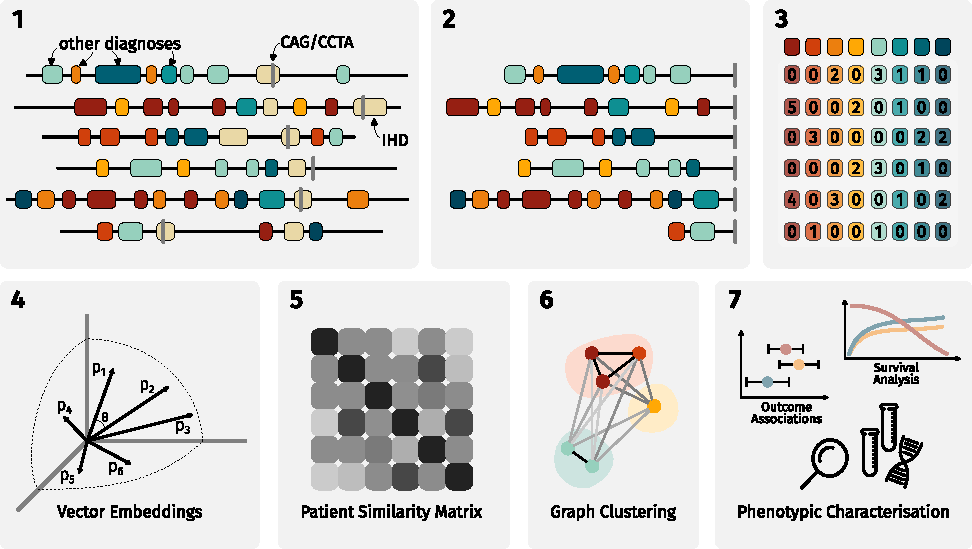
\includegraphics{graphics/clustering-overview.pdf}
    \caption[Overview of Study I Methodology]{%
        Overview of the comorbidity clustering approach in \studyi{},
        detailing the different steps going from \ac{LPR} patient record data
        to identification and characterisation of distinct 
        multimorbidity clusters. 
    }
    \label{fig:dishisclust}
\end{figure*}

The overall methodology employed in this study is illustrated 
in \cref{fig:dishisclust}. In the following, I will be outlining the 
different steps of our comorbidity clustering approach. 

In this study, we represented multimorbidity by constructing patient-level
vectors that aggregated all diagnosis codes assigned up until the index date 
(as illustrated by steps 1 and 2 in \cref{fig:dishisclust}).
We excluded \ac{IHD} codes (\ac{ICD-10}: I20-25) and
codes belonging from chapters XV, XVI, XVII, XIX, XX, and XXI.%
\sidenote{%→
    These chapters are in the Danish \ac{ICD-10} version defined as
    \begin{itemize}[itemsep=1pt, parsep=0pt]
        \item Chapter XV (O00-O99): Pregnancy, childbirth and the puerperium
        \item Chapter XVI (P00-P99): 
            Certain conditions originating in the perinatal period
        \item Chapter XVII (Q00-Q99):
            Congenital malformations, deformations and chromosomal abnormalities
        \item Chapter XIX (S00-T98): 
            Injury, poisoning and certain other consequences of external causes
        \item Chapter XX (X60-Y09): 
            External causes of morbidity and mortality
        \item Chapter XXI (Z00-Z99): 
            Factors influencing health status and contact with health services
    \end{itemize}
}
% ←
In addition, we removed rarely used codes assigned to less than five patients.

The remaining codes were then counted (step 3), 
and embedded in a vector space model 
~\autocite{saltonVector1975}
using \ac{SVD}
~\autocite{golubSingular1971} (step 4).
Next, we used these embedded patient-level vectors 
to create a patient similarity matrix (step 5). 
For this matrix, we used cosine similarity as the similarity measure,
which calculates the cosine of the angle \(\theta\) 
between the embedded vectors.

From the similarity matrix we could then 
construct a patient similarity network,
which is a weighted undirected graph with 
patients as vertices. 
The edges in the graph represents the connections between patients,
which is weighted by the similarity of their respective diagnosis vectors.
As this graph could contain a total of
\num{2609922876} edges, which is computationally intractable, 
we pruned the network by discarding low-similarity edges 
(\(\cos{\theta} \leq 0.3\)) and limited the number of edges
connected to each vertex to the \num{8000} with greatest weight.

Subsequently,
the patient similarity network,
was then subject to cluster analysis,
using the \ac{MCL} algorithm 
~\autocite{vandongenGraph2008}
(step 6). 
The clusters obtained were then characterised (step 7).
This characterisation involved four key aspects 
(i) estimation of \acp{HR} for cluster comparisons using Cox proportional hazards models,
(ii) phenotypic enrichment analysis, 
(iii) examination of clusters based on laboratory test profiles,
and (iv) testing for genetic associations through \acp{PRS}.
In the following I will limit the presentation
of results to aspects (i) and (ii), 
as these are most integral to the study,
and will otherwise refer to the full-length manuscript.

\section{Main Findings}

% \subsection{Cohort Characteristics}
% 
% The study included \num{72249} patients, 
% predominantly male (\qty{63.1}{\percent}), with a mean age of 63.9
% years. 
% The most common inclusion diagnosis was angina pectoris, followed by acute
% myocardial infarction and chronic IHD. The most common comorbidities recorded
% prior to the index \ac{CAG} or \ac{CCTA} is
% hypertension (I10.9), dyslipidemia (E78.0), 
% and non-insulin-dependent diabetes (E11.9).
% The average number of diagnoses in the patient vectors, i.e. prior to index,
% was \num{8.1}. 
% Of the entire cohort, \qty{6.7}{\percent} had no prior diagnoses registered.

\subsection{Cluster Analysis and Outcomes}

%The clustering identified 36 distinct patient subgroups 
%which in total included \qty{94}{\percent} of the cohort. 
%The patients not belonging to a cluster, 
%was primarily those without any registered diagnoses.
%We discarded clusters with a size less than 500 (4 clusters),
%since the goal was to describe the more general patterns of multimorbidity,
%and instead focused the characterisation to the remaining 31 clusters.

The clustering resulted in 31 distinct patient subgroups, 
each characterised by specific patterns of multimorbidity.
We incorporated cluster membership in Cox regression models, 
which was further adjusted for sex and age. 
This was to obtain estimates for the risk associated with the comorbidity
profiles in each cluster, beyond those patterns primarily dependent on
age or sex.
The \acp{HR} were estimated 
by contrasting each single cluster against all others.
The size of clusters, mean age at index, and average propotion of males, 
and the adjusted \acp{HR} for the two outcomes, are
depicted in \cref{fig:cluster-results}.

\begin{figure*}[t!]% →
    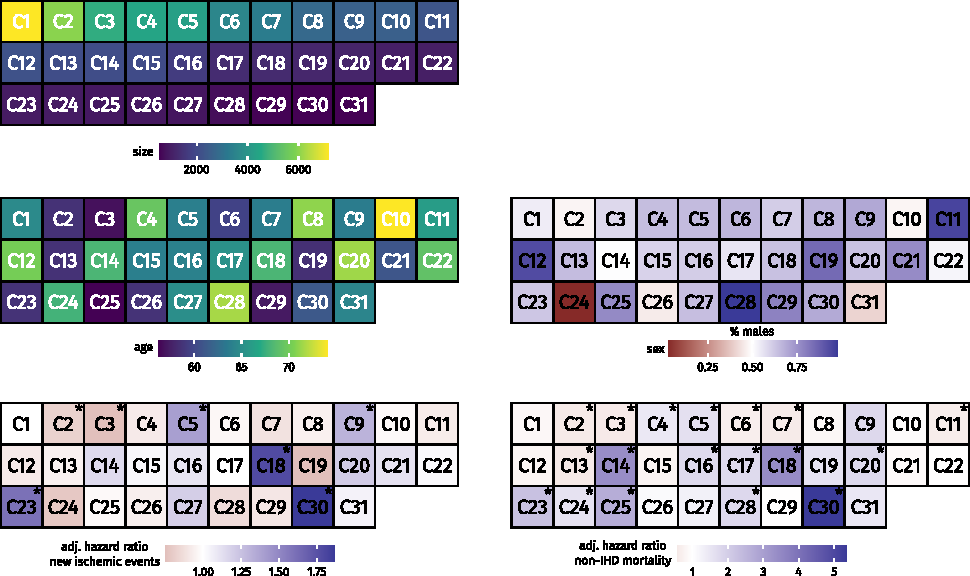
\includegraphics{graphics/clustering-results.pdf}
    \caption[Cluster Characteristics and Outcomes][0em]{%
        Cluster characteristics and adjusted hazard ratios.
        The first panel,
        from top-left to bottom-right,
        shows the number
        of patients in each cluster, 
        arranged according to their respective sizes.
        This ordering is maintained in subsequent panels.
        The second panel shows the average age at the index \ac{CAG}/\ac{CCTA},
        ranging from \qty{56.2}{years} (C25) to \qty{74.2}{years} (C10).
        The third panel shows the sex distribution in each cluster,
        using fill color to indicate the proportion of males;
        red for clusters with more than \qty{50}{\percent} females,
        and blue for those with more than \qty{50}{\percent} males.
        The fourth and fifth panels shows the adjusted hazard ratios
        for new ischemic events and non-\ac{IHD} mortality, respectively.
        Here, clusters with a red fill indicate an \ac{HR} below one,
        while those with a blue fill have an \ac{HR} above one.
        Clusters with a hazard ratio significantly different from
        one are marked with an asterisk (\(*\)).
    }
    \label{fig:cluster-results}
\end{figure*}% ←

Our analysis revealed that
certain clusters had significantly different risks compared to others.
Comorbidity profiles within five clusters (C5, C9, C18, C23, C30) were
associated with a significantly increased risk of new ischemic events.
Conversely, profiles in two clusters (C2, C3) were associated with a 
significantly reduced risk of these events. 
Twelve clusters (C4, C5, C14, C16, C17, C18, C20, C23, C24, C25,
C28, C30) had profiles associated with a significantly higher risk 
of non-\ac{IHD} mortality. 
In contrast, six clusters (C2, C3, C6, C7, C11, C13) had
profiles that were linked to a significantly lower risk of 
non-\ac{IHD} mortality.
Of note, four of the five cluster profiles with an increased risk of 
new ischemic events also exhibited an increased risk of 
non-\ac{IHD} mortality. 

\subsection{Phenotypic Characterisation of Clusters}

\begin{figure*}[tbp]
    \includegraphics[clip=false, trim=6mm 5mm 0 4mm]%
        {graphics/cluster-summary.pdf}
    \caption[Overview of Cluster Phenotypes]{%
        From manual review of the between-cluster enrichment of 
        diagnosis codes, we assigned each cluster a label based
        on its most prevalent codes.
        To aid the intrepretation, the clusters were further organized by 
        consideration of their estimated hazard ratios 
        and shared diagnostic similarity.
        Clusters marked with \uporange{} or \upblue{} have a 
        significantly increased risk of new ischemic events
        and non-\ac{IHD} mortality, respectively.
        Conversely, \downorange{} or \downblue{} marks those with
        a significantly decreased risk.
        A single arrow indicates the direction of the effect 
        and that the association was not found to be significant.

    }
    \label{fig:cluster-summary}
\end{figure*}

% To describe the patterns associated with increased or 
% decreased risks, we further characterised the clusters
% and summarise our key findings here.

As a first step, we evaluated the intra-cluster prevalence of all unique diagnosis
codes (\num{3046} in total) within patient vectors. 
These prevalences was then compared with the average prevalences
across all clusters by calculating \ac{OE}-ratios, 
to pinpoint \ac{ICD-10} codes that were disproportionately represented 
in various clusters.  
The top ten most overrepresented or underrepresented codes for each
cluster are detailed in supplementary tables 5A and 5B of the manuscript
(\cref{chap:study1-paper}).

We conducted a manual review of these findings, assigning a label to each
cluster based on the associated codes. Given that multiple codes could pertain
to a single cluster, these labels are not definitive but offer a general
overview, as depicted in \cref{fig:cluster-summary}. 
Furthermore, in \cref{fig:cluster-summary}, we organise the
clusters by both their common traits and the hazard ratios 
derived from the Cox analyses.

\section{Interpretation}

From \cref{fig:cluster-summary}, 
we see that the five clusters (C5, C9, C18, C23, C30) with a 
significantly increased risk of both new ischemic events and non-\ac{IHD} mortality
were characterised by the presence of important prognostic comorbidities in \ac{IHD}:
diabetes, peripheral atherosclerosis, heart failure, 
and chronic kidney disease. 

Both diabetes and chronic kidney disease 
are highlighted as important non-cardiovascular
comorbidities in the 2019 \acsu{ESC} guidelines for chronic coronary syndromes,
and both peripheral artery disease and renal dysfunction is explicitly
described as comorbidities that negatively impact prognosis.%
\sidecite[15em]{knuuti20192020}
Heart failure, 
also known to affect prognosis and included in clinical guidelines,
is, for example, included as one of eight carefully selected predictors
in the widely used \acsfont{GRACE} risk and mortality calculator.%
\sidecite[13em]{foxShould2014}
This showcases that our framework is able to identify known comorbidites
that affect the clinical course of cardiovascular disease.
In addition, it further emphasizes the significance of these 
comorbidities and the broader concept of considering
comorbidity in clinical assessment of \ac{IHD}.

We did not identify other clusters with comorbidity profiles
that significicantly increased the risk of new ischemic events,
however, both the second and third largest clusters (C2 and C3)
were found to have comorbidities associated with a significant decreased risk
of both new ischemic events and non-\ac{IHD} mortality.
Cluster C2 is characterised by the presence of codes 
for both gallstones (K80) and abdominal pain (R10).
Cluster C3 relates to symptom codes (R00-R99),
with high \ac{OE}-ratios for
{pain in throat and chest} (R07.9), 
{other chest pain} (R07.3), 
and {muscle strain} (M62.6).

It is interesting that the second largest cluster (C2)
is characterised by gallstones as a comorbid condition.
Many studies have previously reported a link between
gallstones and ischemic heart disease,
\autocite{zhengGallstones2016}
\autocite{upalaGallstone2017}
\autocite{wirthPresence2015}
however, the underlying reasons for this association remain
somewhat unclear and it is uncertain the link is causal.
It is known that the two diseases shares pathogenicity factors,
which include hypercholesterolemia, diabetes, and hypertension,
so parts of the pathological mechanism is likely shared.
\autocite{zhengGallstones2016}

In our study, focusing on patients with incident \ac{IHD},
the presence of gallstones appear to positively affect prognosis.
A possible explanation is that acute symptoms of gallstone disease
can immitate heart disease symptoms, and thus, the cluster could be 
enriched for patients that may not have \ac{IHD} to begin with.
This area warrants further investigation to better understand these connections
and their implications for clinical practice.

Two clusters were characterised by the co-occurence of cancer comorbidities.
Clusters C24 and C28 were enriched for breast and prostate cancer, 
respectively.
Our current methodology does not distinguish between active cancer
or if the patient has been cured, which represents a key limitation
of the approach.
However, both clusters were found to have an increased risk of 
non-\ac{IHD} mortality.

In patients with active cancer,
the management of \ac{IHD}, and specifically \ac{ACS}, 
is challenged by increased risk of bleeding,
low platelet count, and increased thrombotic risk.
~\autocite{byrne20232023}
Furthermore, 
many chemotherapeutic agents have cardiotoxic side effects,
as discussed in a 2016 \ac{ESC} position paper on the 
cardivascular toxicity of cancer treatment.
~\autocite{zamorano20162016}
Moreover,
studies indicate that radiotherapy breast cancer
is associated with an increased risk of developing \ac{IHD}, 
in a dose-dependent manner.
~\autocite{darbyRisk2013}
This underscores the complex balancing act involved in concurrently managing
both conditions, where the treatment of one disease can potentially exacerbate
the other.

\section{Conclusion}

In this study, we presented a large-scale data-driven approach
for analysis of comorbidity patterns in more than \num{70000} adult 
patients with incident \ac{IHD}.
We took a hypothesis-free approach and used a broad definition of 
multimorbidity, including more than \num{3000} different \ac{ICD-10} codes in
the decription of prior and coexisting comorbidities in \ac{IHD}.
Using unsupervised clustering, we identified disctinct groups of patients 
each characterised by specific patterns of multimorbidity and associated
risks of both disease progression and mortality from unrelated causes.

Mapping out the landscape of multimorbidities in a real-world cohort of 
patients with \ac{IHD}, could inform clinical managment and could serve
as a tool for identification of comorbidity combinations for which
current clinical knowledge is currently limited.
Strict inclusion and exclusion criteria in many \acp{RCT} 
potentially limit the applicability of existing \ac{IHD} 
management guidelines on patients with pronounced multimorbidity.
~\autocite{richKnowledge2016}
To adress such limitations, an important first step is to obtain an overview
of the specific patterns of multimorbidity associated with \ac{IHD}.
